%%%%%%%%%%%%%%
%% Run LaTeX on this file several times to get Table of Contents,
%% cross-references, and citations.

%% If you have font problems, you may edit the w-bookps.sty file
%% to customize the font names to match those on your system.

%% w-bksamp.tex. Current Version: Feb 16, 2012
%%%%%%%%%%%%%%%%%%%%%%%%%%%%%%%%%%%%%%%%%%%%%%%%%%%%%%%%%%%%%%%%
%
%  Sample file for
%  Wiley Book Style, Design No.: SD 001B, 7x10
%  Wiley Book Style, Design No.: SD 004B, 6x9
%
%
%  Prepared by Amy Hendrickson, TeXnology Inc.
%  http://www.texnology.com
%%%%%%%%%%%%%%%%%%%%%%%%%%%%%%%%%%%%%%%%%%%%%%%%%%%%%%%%%%%%%%%%

%%%%%%%%%%%%%
% 7x10
%\documentclass{wileySev}

% 6x9

\documentclass{wileysix}
\UseRawInputEncoding
\usepackage{graphicx}
\usepackage{listings}

\usepackage{float}

\usepackage{color}
 
\definecolor{codegreen}{rgb}{0,0.6,0}
\definecolor{codegray}{rgb}{0.5,0.5,0.5}
\definecolor{codepurple}{rgb}{0.58,0,0.82}
\definecolor{backcolour}{rgb}{0.95,0.95,0.92}
 
\lstdefinestyle{mystyle}{
    backgroundcolor=\color{backcolour},   
    commentstyle=\color{codegreen},
    keywordstyle=\color{magenta},
    numberstyle=\tiny\color{codegray},
    stringstyle=\color{codepurple},
    basicstyle=\footnotesize,
    breakatwhitespace=false,         
    breaklines=true,                 
    captionpos=b,                    
    keepspaces=true,                 
    numbers=left,                    
    numbersep=5pt,                  
    showspaces=false,                
    showstringspaces=false,
    showtabs=false,                  
    tabsize=2,
    language=sh
}
 
\lstset{style=mystyle}

%%%%%%%
%% for times math: However, this package disables bold math (!)
%% \mathbf{x} will still work, but you will not have bold math
%% in section heads or chapter titles. If you don't use math
%% in those environments, mathptmx might be a good choice.

% \usepackage{mathptmx}

% For PostScript text
\usepackage{w-bookps}

%%%%%%%%%%%%%%%%%%%%%%%%%%%%%%%%%%%%%%%%%%%%%%%%%%%%%%%%%%%%%%%%
%% Other packages you might want to use:

% for chapter bibliography made with BibTeX
% \usepackage{chapterbib}

% for multiple indices
% \usepackage{multind}

% for answers to problems
% \usepackage{answers}

%%%%%%%%%%%%%%%%%%%%%%%%%%%%%%
%% Change options here if you want:
%%
%% How many levels of section head would you like numbered?
%% 0= no section numbers, 1= section, 2= subsection, 3= subsubsection
%%==>>
\setcounter{secnumdepth}{3}

%% How many levels of section head would you like to appear in the
%% Table of Contents?
%% 0= chapter titles, 1= section titles, 2= subsection titles, 
%% 3= subsubsection titles.
%%==>>
\setcounter{tocdepth}{2}

%% Cropmarks? good for final page makeup
%% \docropmarks

%%%%%%%%%%%%%%%%%%%%%%%%%%%%%%
%
% DRAFT
%
% Uncomment to get double spacing between lines, current date and time
% printed at bottom of page.
% \draft
% (If you want to keep tables from becoming double spaced also uncomment
% this):
% \renewcommand{\arraystretch}{0.6}
%%%%%%%%%%%%%%%%%%%%%%%%%%%%%%

%%%%%%% Demo of section head containing sample macro:
%% To get a macro to expand correctly in a section head, with upper and
%% lower case math, put the definition and set the box 
%% before \begin{document}, so that when it appears in the 
%% table of contents it will also work:

\newcommand{\VT}[1]{\ensuremath{{V_{T#1}}}}

%% use a box to expand the macro before we put it into the section head:

\newbox\sectsavebox
\setbox\sectsavebox=\hbox{\boldmath\VT{xyz}}

%%%%%%%%%%%%%%%%% End Demo


\begin{document}


\booktitle{Dasar-dasar Python}
\subtitle{}

\authors{Rolly M. Awangga\\
\affil{Informatics Research Center}
%Floyd J. Fowler, Jr.\\
%\affil{University of New Mexico}
}

\offprintinfo{Cerdas Menguasai Git, First Edition}{Rolly M. Awangga}

%% Can use \\ if title, and edition are too wide, ie,
%% \offprintinfo{Survey Methodology,\\ Second Edition}{Robert M. Groves}

%%%%%%%%%%%%%%%%%%%%%%%%%%%%%%
%% 
\halftitlepage

\titlepage


\begin{copyrightpage}{2019}
%Survey Methodology / Robert M. Groves . . . [et al.].
%\       p. cm.---(Wiley series in survey methodology)
%\    ``Wiley-Interscience."
%\    Includes bibliographical references and index.
%\    ISBN 0-471-48348-6 (pbk.)
%\    1. Surveys---Methodology.  2. Social 
%\  sciences---Research---Statistical methods.  I. Groves, Robert M.  II. %
%Series.\\
%
%HA31.2.S873 2007
%001.4'33---dc22                                             2004044064
\end{copyrightpage}

\dedication{`Jika Kamu tidak dapat menahan lelahnya belajar, 
Maka kamu harus sanggup menahan perihnya Kebodohan.'
~Imam Syafi'i~}

\begin{contributors}
\name{Rolly Maulana Awangga,} Informatics Research Center., Politeknik Pos Indonesia, Bandung,
Indonesia



\end{contributors}

\contentsinbrief
\tableofcontents
\listoffigures
\listoftables
\lstlistoflistings


\begin{foreword}
Sepatah kata dari Kaprodi, Kabag Kemahasiswaan dan Mahasiswa
\end{foreword}

\begin{preface}
Buku ini diciptakan bagi yang awam dengan git sekalipun.

\prefaceauthor{R. M. Awangga}
\where{Bandung, Jawa Barat\\
Februari, 2019}
\end{preface}


\begin{acknowledgments}
Terima kasih atas semua masukan dari para mahasiswa agar bisa membuat buku ini 
lebih baik dan lebih mudah dimengerti.

Terima kasih ini juga ditujukan khusus untuk team IRC yang 
telah fokus untuk belajar dan memahami bagaimana buku ini mendampingi proses 
Intership.
\authorinitials{R. M. A.}
\end{acknowledgments}

\begin{acronyms}
\acro{ACGIH}{American Conference of Governmental Industrial Hygienists}
\acro{AEC}{Atomic Energy Commission}
\acro{OSHA}{Occupational Health and Safety Commission}
\acro{SAMA}{Scientific Apparatus Makers Association}
\end{acronyms}

\begin{glossary}
\term{git}Merupakan manajemen sumber kode yang dibuat oleh linus torvald.

\term{bash}Merupakan bahasa sistem operasi berbasiskan *NIX.

\term{linux}Sistem operasi berbasis sumber kode terbuka yang dibuat oleh Linus Torvald
\end{glossary}

\begin{symbols}
\term{A}Amplitude

\term{\hbox{\&}}Propositional logic symbol 

\term{a}Filter Coefficient

\bigskip

\term{\mathcal{B}}Number of Beats
\end{symbols}

\begin{introduction}

%% optional, but if you want to list author:

\introauthor{Rolly Maulana Awangga, S.T., M.T.}
{Informatics Research Center\\
Bandung, Jawa Barat, Indonesia}

Pada era disruptif  \index{disruptif}\index{disruptif!modern} 
saat ini. git merupakan sebuah kebutuhan dalam sebuah organisasi pengembangan perangkat lunak.
Buku ini diharapkan bisa menjadi penghantar para programmer, analis, IT Operation dan Project Manajer.
Dalam melakukan implementasi git pada diri dan organisasinya.

Rumusnya cuman sebagai contoh aja biar keren\cite{awangga2018sampeu}.

\begin{equation}
ABC {\cal DEF} \alpha\beta\Gamma\Delta\sum^{abc}_{def}
\end{equation}

\end{introduction}

%%%%%%%%%%%%%%%%%%Isi Buku_

\chapter{Python}
\chapter{\textit{Python}}

\section{Sejarah \textit{Python}}
Python merupakan bahasa pemrograman tingkat tinggi yang dapat digunakan banyak hal, \textit{Python} awalnya dirancang oleh \textbf{Guido van Rossum} pada tahun 1980 yang mana nama \textit{Python} sebelum sebesar sekarang yaitu \textit{ABC Programming Language} yang dijalankan di sistem operasi bernama \textit{Amoeba Operating System}. Guido merasakan kehebatan dan kemampuan serta fitur yang berada pada bahasa pemrograman ABC ini sehingga Guido mengambil siktaks-sintaks yang berada pada bahasa pemrograman ABC ini, tentu saja banyak komplain yang berdatangan sehingga Guido terus melakukan perbaikan pada bahasa pemrograman yang sedang ia buat kala itu. Lalu, disinilah nama \textit{Python} muncul dimuka bumi sebagai bahasa pemrograman, disaat Guido sedang menonton televisi dan menemukan kata '\textit{Monty Python's Flying Circus}'.

Bahasa \textit{Python} secara resmi dirilis pada tahun 1991, saat rilis pertama kali semua orang terkejut dengan sintaks yang dimiliki oleh \textit{Python} ketika dibandingkan dengan bahasa lain seperti \textit{Java, C, C++}, dan lain-lain pengekspresian bahasa ini cukup sederhana. Tujuan dari dibuatnya bahasa pemrograman ini adalah untuk mempermudah dalam membaca sebuah kode dari penulisan sintaks dan produktivitas dalam hal pengembangan tingkat lanjut.

\section{Perbedaan \textit{Python 2.x} dan \textit{Python 3.x}}
Banyak perbedaan yang akan kita temui jika kita dahulu pernah menggunakan \textit{python} versi 2.x cukup lama sehingga berpindah ke versi 3.x, berikut contoh perbedaan pada \textit{python} versi 2.x dan 3.x yang sangat penting untuk diketahui:

\begin{enumerate}

\item Perintah \textbf{print}
Perbedaan perintah \textit{print} pada dua versi ini adalah python 2.x tidak memakai kurung dan 3.x memakai kurung untuk perintah \textit{print} bisa dilihat pada gambar ~\ref{print} dan \ref{printnano}

\begin{figure}[H]
\centering
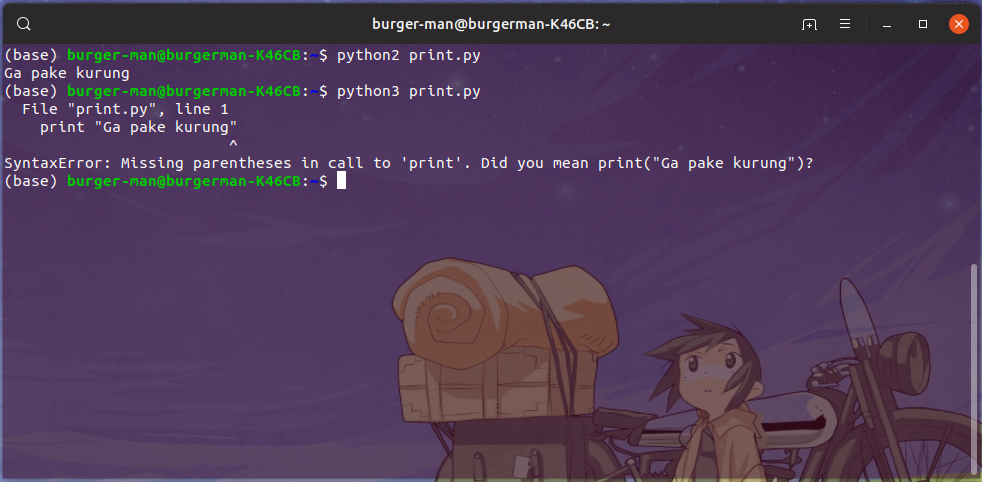
\includegraphics[width=1\textwidth]{figures/print.png}
\caption{Gambar hasil print}
\label{print}
\end{figure}

\begin{figure}[H]
\centering
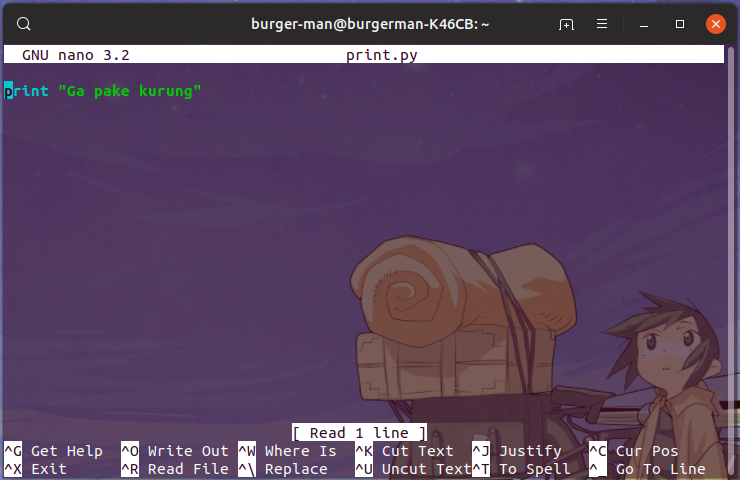
\includegraphics[width=1\textwidth]{figures/printnano.png}
\caption{Gambar perintah print}
\label{printnano}
\end{figure}

\item Perintah pembagian \textbf{\textit{integer}}
Hasil dari perintah pembagian cukup jelas berbeda yang mana versi 2.x tidak secara mendetail untuk hasilnya sehingga angka yang dihasilkan bilangan \textbf{\textit{integer}} sedangkan versi 3.x bertipe \textbf{\textit{float}} perbedaannya bisa dilihat pada gambar \ref{div} dan \ref{divnano}.

\begin{figure}[H]
\centering
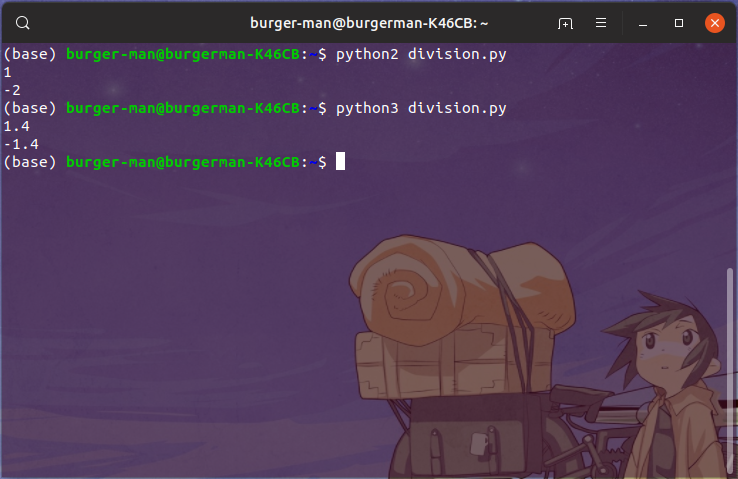
\includegraphics[width=1\textwidth]{figures/div.png}
\caption{Gambar hasil pembagian}
\label{div}
\end{figure}

\begin{figure}[H]
\centering
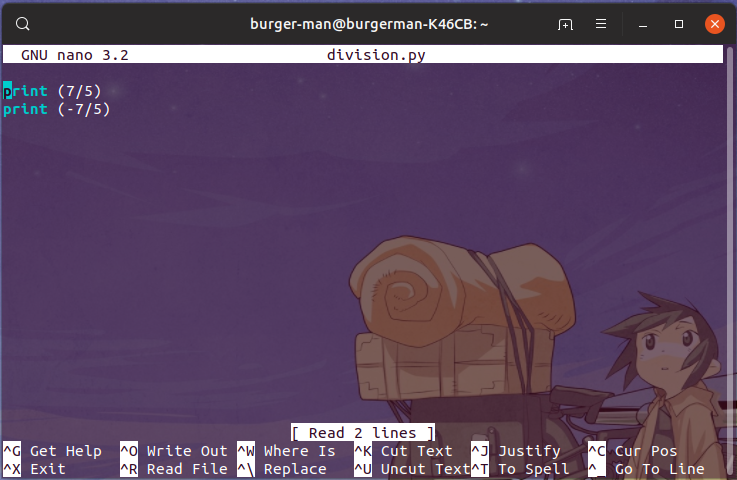
\includegraphics[width=1\textwidth]{figures/divnano.png}
\caption{Gambar perintah pembagian}
\label{divnano}
\end{figure}

\item \textit{\textbf{Try and Except}}
Perbedaan pada \textit{try and expcept} hanya berbeda di penggunaan \textbf{,} untuk versi 2.x dan \textbf{as} untuk versi 3.x.

\begin{figure}[H]
\centering
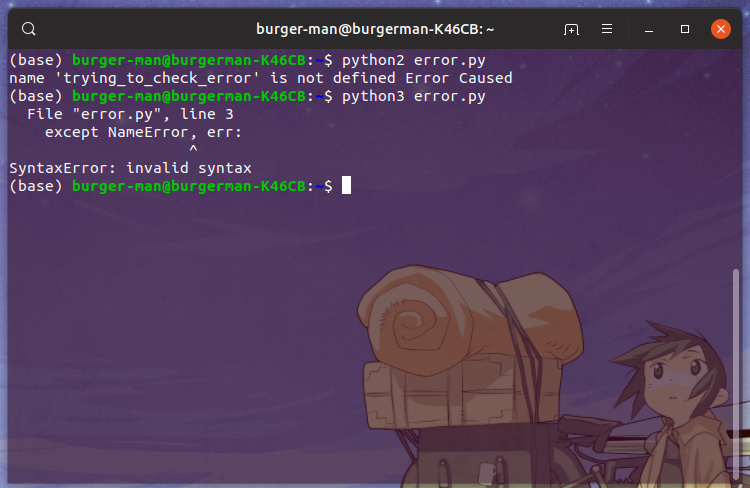
\includegraphics[width=1\textwidth]{figures/error.png}
\caption{Gambar hasil error}
\label{error}
\end{figure}

\begin{figure}[H]
\centering
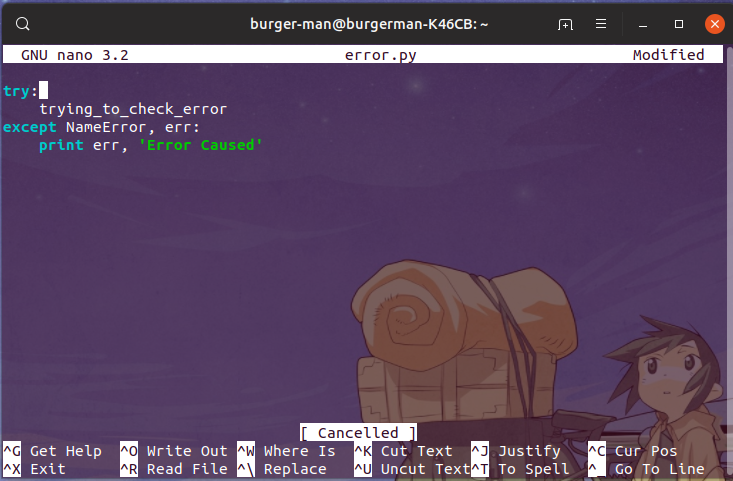
\includegraphics[width=1\textwidth]{figures/errornano.png}
\caption{Gambar perintah error}
\label{errornano}
\end{figure}

\item \textbf{\textit{Looping}}
Perbedaan pada looping hanya saja versi 3.x tidak bisa menggunakan sintaks \textbf{\textit{xrange}} lagi.

\begin{figure}[H]
\centering
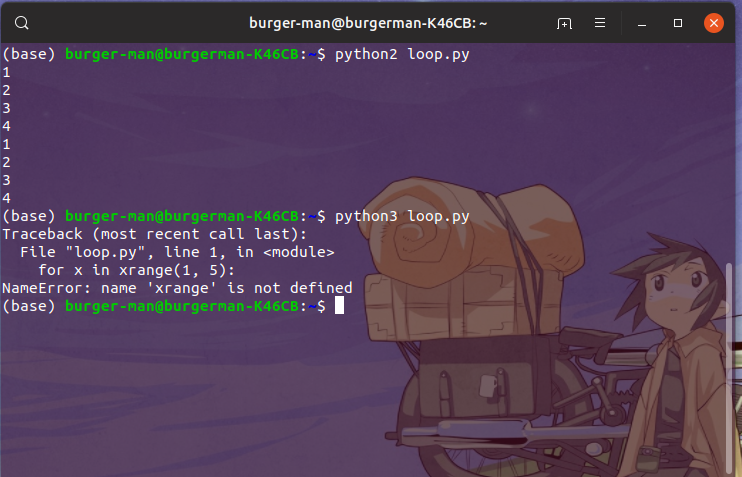
\includegraphics[width=1\textwidth]{figures/loop.png}
\caption{Gambar hasil looping}
\label{loop}
\end{figure}

\begin{figure}[H]
\centering
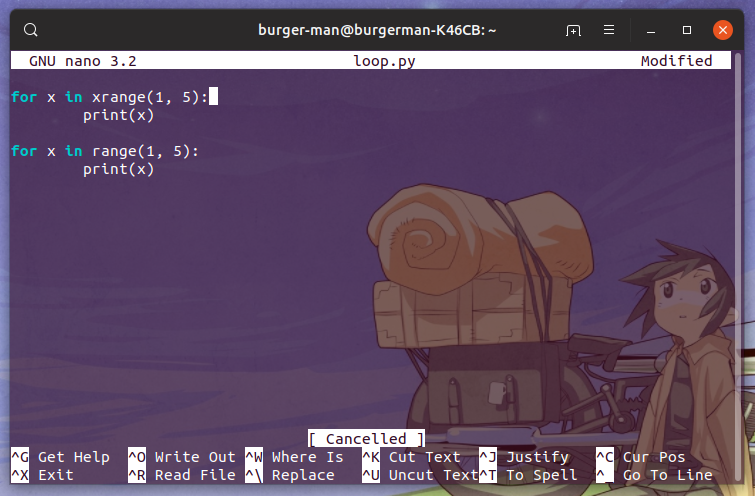
\includegraphics[width=1\textwidth]{figures/loopnano.png}
\caption{Gambar perintah looping}
\label{loopnano}
\end{figure}

\item \textbf{\textit{Unicode}}
Unicode ini cukup penting karena kita mengetahui bagaimana setiap versi merespons setiap unicode yang diberikan.

\begin{figure}[H]
\centering
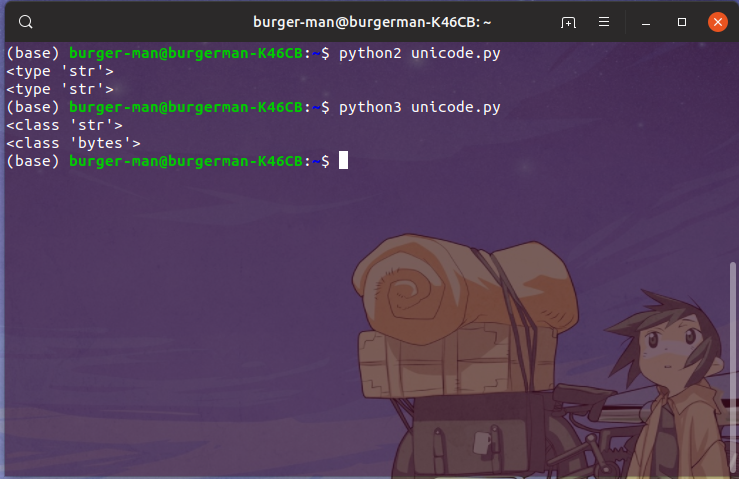
\includegraphics[width=1\textwidth]{figures/unicodebytes.png}
\caption{Gambar hasil unicode (bytes)}
\label{unibytes}
\end{figure}

\begin{figure}[H]
\centering
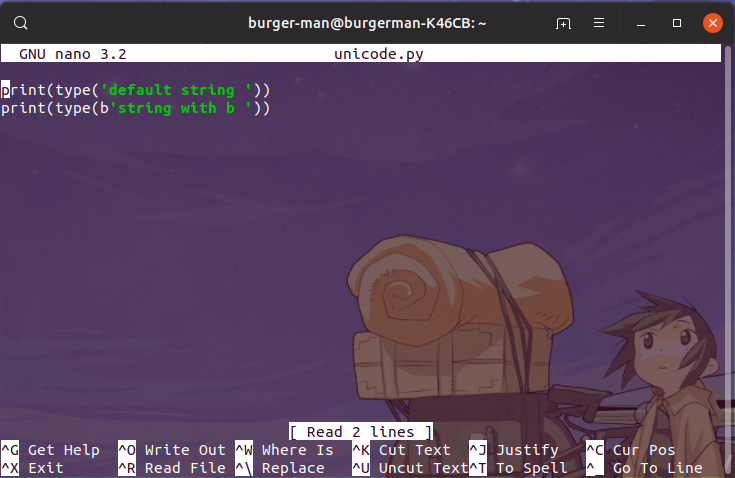
\includegraphics[width=1\textwidth]{figures/unicodebytesnano.png}
\caption{Gambar perintah unicode (bytes)}
\label{unibytesnano}
\end{figure}
Pada gambar ~\ref{unibytes} terlihat jelas bahwa perintah \textbf{\textit{bytes}} hanya direspon pada versi 3.x sedangkan versi 2.x merespon \textbf{\textit{string}}

\begin{figure}[H]
\centering
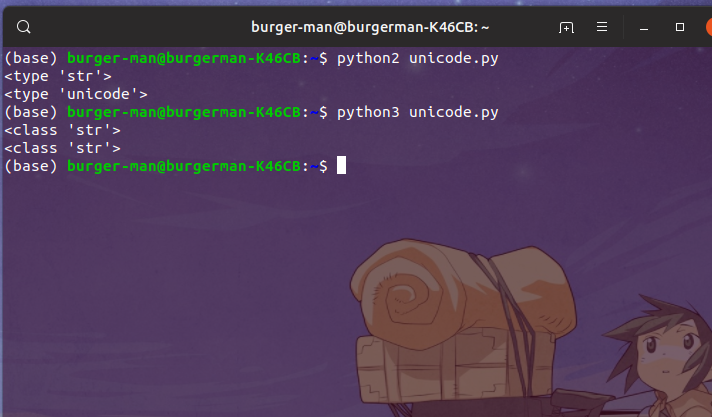
\includegraphics[width=1\textwidth]{figures/unicodeuni.png}
\caption{Gambar hasil unicode}
\label{unicodeuni}
\end{figure}

\begin{figure}[H]
\centering
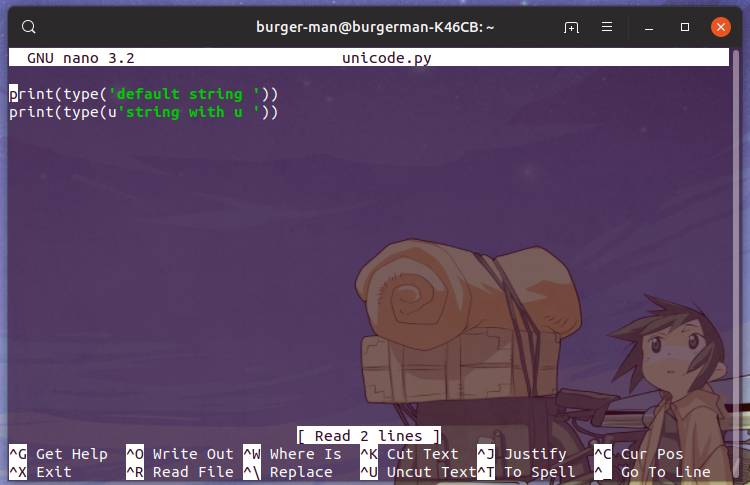
\includegraphics[width=1\textwidth]{figures/unicodeuninano.png}
\caption{Gambar perintah unicode}
\label{unicodeuninano}
\end{figure}

\end{enumerate}

\section{Installasi Python}
Untuk installasi kali ini akan bagi menjadi dua sistem operasi yaitu Windows (Windows 10), dan Linux (Ubuntu 19.04). Installasi menggunakan \textit{environtment} Anaconda sebagai installasi \textit{python}. Anaconda merupakan \textit{environment open-source} untuk bahasa pemrograman \textit{Python}, dan \textit{R} berfungsi untuk memanajemen penggunaan \textit{package} pada \textit{python} dan \textit{R}.

\subsection{Windows (Windows 10)}
Hal yang harus diperhatikan sebelum melakukan instalasi \textit{Anaconda Python}
\begin{enumerate}
 \item Perhatikan versi dari sistem operasi yang digunakan (versi 32bit atau 64bit)
 \item Download file anaconda yang sesuai dengan versi sistem operasi (32bit atau 64bit)
 \item \textit{Download Anaconda Python} https://www.anaconda.com/distribution/
\end{enumerate}

Berikut langkah-langkah instalasi anaconda.
\begin{enumerate}
\item Buka aplikasi \textit{installer Anaconda} tersebut lalu akan muncul  gambar \textit{installer anaconda}.
\begin{figure}[H]
        \centerline{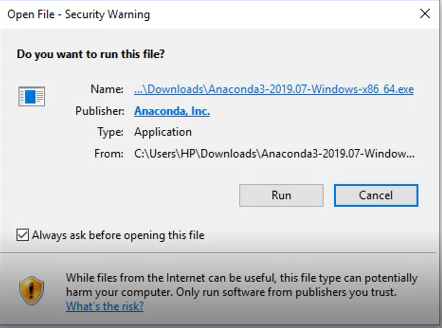
\includegraphics[scale=0.5]{figures/1}}
        \caption{Run Setup Anaconda}
		\label{langkah1}
\end{figure}

\item Tunggu hingga \textit{setup loading} selesai
\begin{figure}[H]
        \centerline{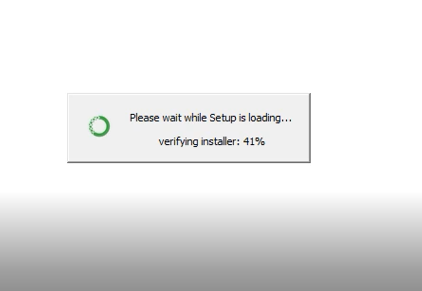
\includegraphics[scale=0.5]{figures/2}}
        \caption{Setup Loading}
		\label{langkah2}
\end{figure}


\item Jika \textit{setup loading} telah selesai, maka klik \textit{next}
\begin{figure}[H]
        \centerline{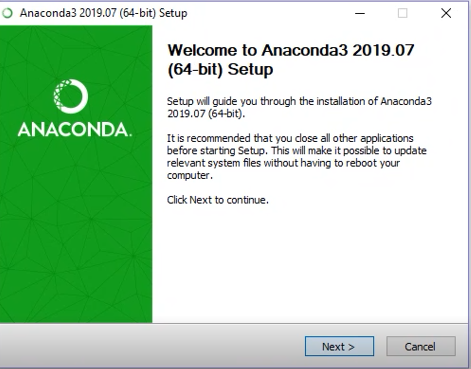
\includegraphics[scale=0.5]{figures/3}}
        \caption{Welcome to Anaconda Setup}
		\label{langkah2}
\end{figure}


\item Pada \textit{License Agreement} klik \textit{I Agree}
 gambar \textit{License Agreement}.

\begin{figure}[H]
    \centering
    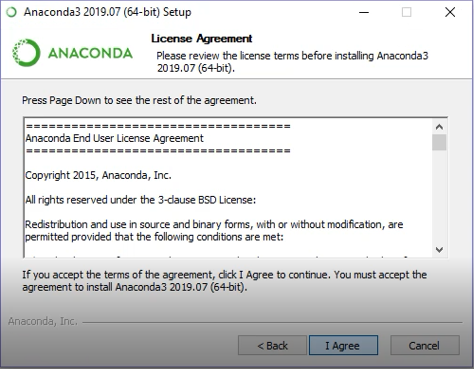
\includegraphics[scale=0.5]{figures/4}
    \caption{\textit{License Agreement}}
    \label{Figureanaconda3}
\end{figure}


\item Kemudian pilih \textit{Just Me(Recomended)} agar sesuai dengan komputer yang digunakan, kemudian klik \textit{next}
 gambar \textit{Just Me(recomended)}.

\begin{figure}[H]
    \centering
    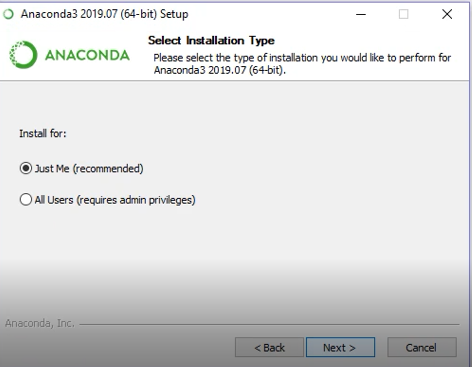
\includegraphics[scale=0.5]{figures/5}
    \caption{\textit{Just Me(recomended)}}
    \label{Figureanaconda4}
\end{figure}


\item Kemudian pilih lokasi tempat \textit{menginstall anaconda}
 gambar \textit{Pilih lokasi}.

\begin{figure}[H]
    \centering
    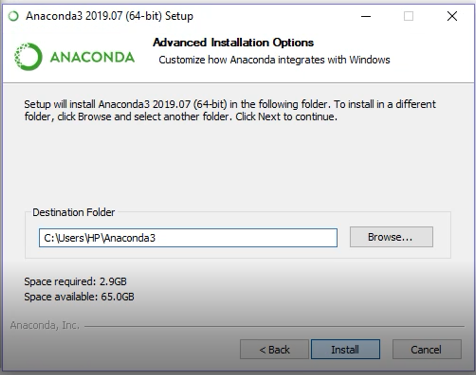
\includegraphics[scale=0.5]{figures/6}
    \caption{\textit{Pilih lokasi}}
    \label{Figureanaconda5}
\end{figure}

\item Kemudian centang \textit{Add Anaconda to my Path environtment variable}, agar saat \textit{menginstall selenium} langsung ke \textit{path anaconda} tidak ke aplikasi yang lain. Klik \textit{install}
 gambar \textit{Centang Anaconda to my PATH}.

\begin{figure}[H]
    \centering
    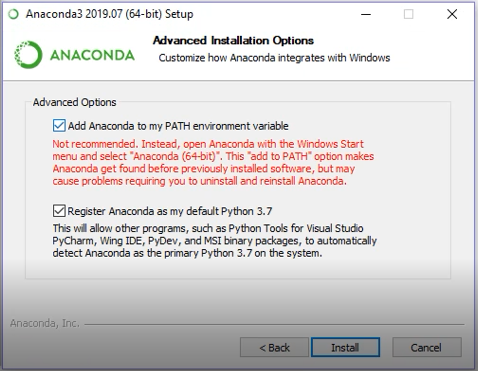
\includegraphics[scale=0.5]{figures/7}
    \caption{\textit{Centang Anaconda to my PATH}}
    \label{Figureanaconda6}
\end{figure}

\item Tunggu sampai proses \textit{installasi} selesai
 gambar \textit{Installation Complete}.

\begin{figure}[H]
    \centering
    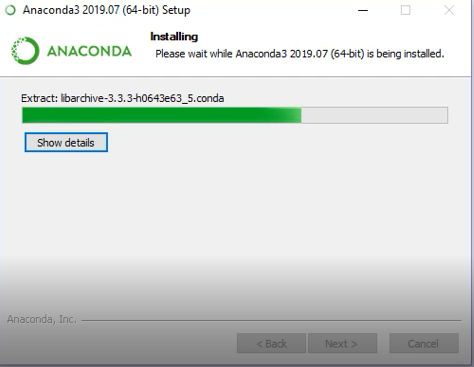
\includegraphics[scale=0.5]{figures/8}
    \caption{\textit{Installation Complete}}
    \label{Figureanaconda7}
\end{figure}

\item Apabila instalasi telah selesai klik \textit{next}
\begin{figure}[H]
    \centering
    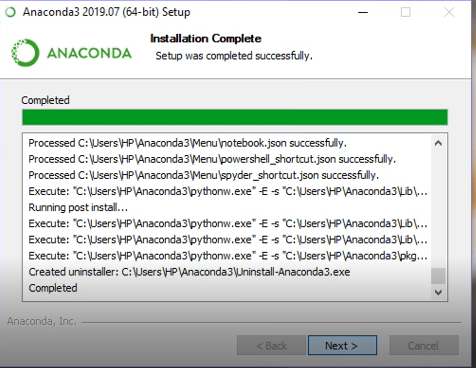
\includegraphics[scale=0.5]{figures/9}
    \caption{\textit{Installation Complete}}
    \label{Figureanaconda8}
\end{figure}

\item klik \textit{next}
\begin{figure}[H]
    \centering
    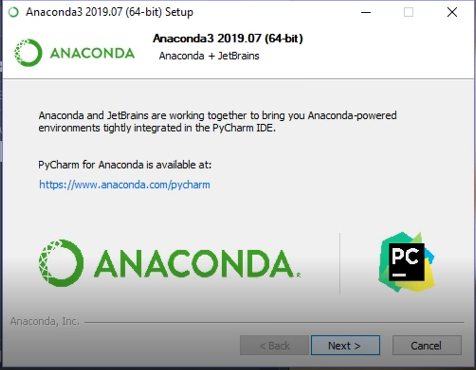
\includegraphics[scale=0.5]{figures/10}
    \caption{\textit{Anaconda+JetBrains}}
    \label{Figureanaconda70}
\end{figure}

\item Jika sudah klik \textit{finish}
 gambar \textit{Thanks fo install Anaconda}.

\begin{figure}[H]
    \centering
    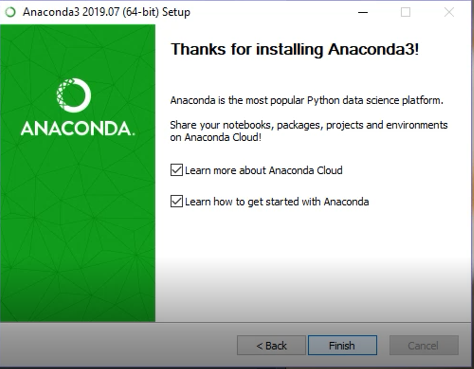
\includegraphics[scale=0.5]{figures/11}
    \caption{\textit{Thanks for install Anaconda}}
    \label{Figureanaconda70}
\end{figure}
\end{enumerate}

\section{Instalasi Pip}
\subsection{Windows (Windows 10)}
\begin{enumerate}
\item buka anaconda promt
\item ketikkan conda install -c anaconda pip
\begin{figure}[H]
    \centering
    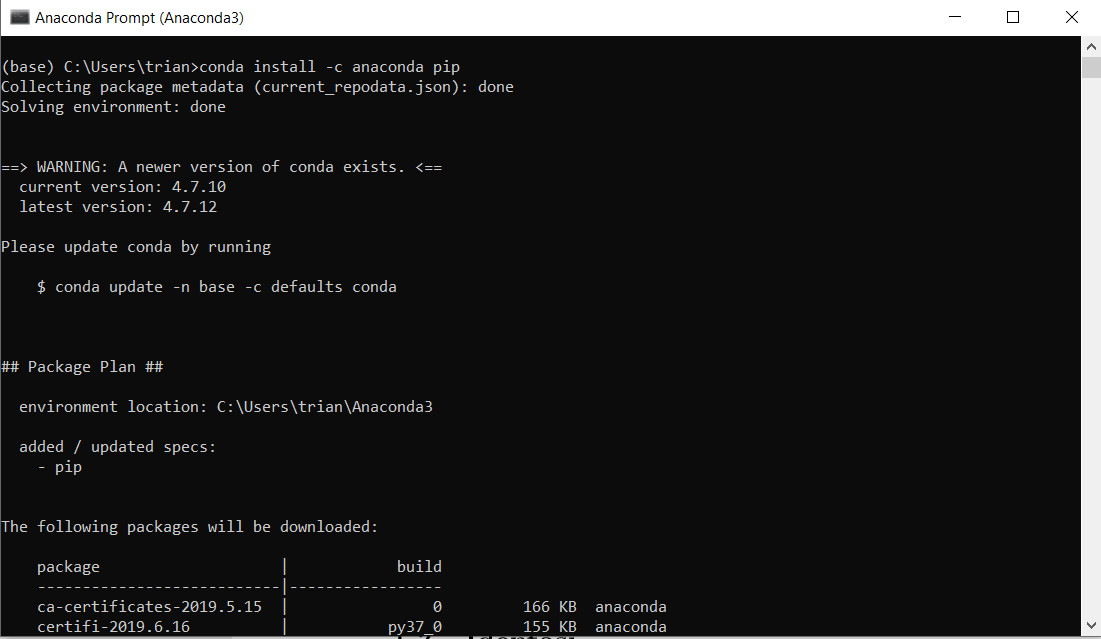
\includegraphics[scale=0.5]{figures/installpip (2)}
    \caption{\textit{Install pip}}
    \label{Figureanaconda70}
\end{figure}
\item ketik y, lalu enter. Tunggu hingga proses instalasi selesai.
\begin{figure}[H]
    \centering
    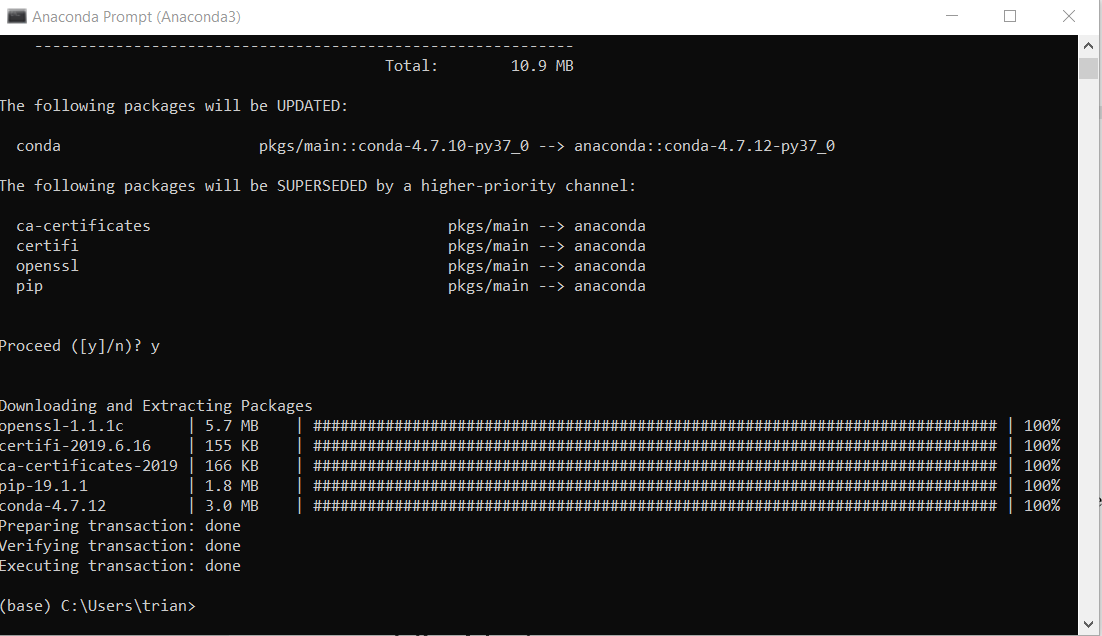
\includegraphics[scale=0.5]{figures/pipselesai}
    \caption{\textit{Install pip Selesai}}
    \label{Figureanaconda70}
\end{figure}
\item jika telah selesai, lakukan pengecekan versi pip dengan mengetikkan pip -V
\begin{figure}[H]
    \centering
    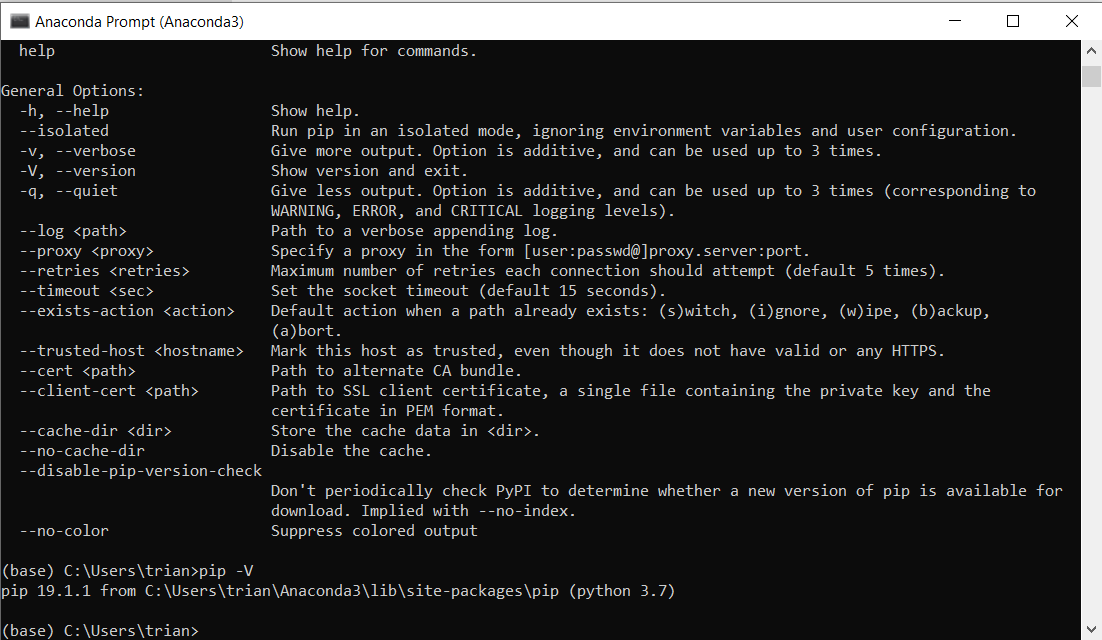
\includegraphics[scale=0.5]{figures/pipversion}
    \caption{\textit{Melihat Versi pip}}
    \label{Figureanaconda70}
\end{figure}

\end{enumerate}

\subsection{Linux (Ubuntu 19.04)}
\begin{enumerate}

\item pertama kita buka terminal kita lalu ketikkan perintah \textbf{sudo apt install python3-pip -y} untuk pip3 dan \textbf{sudo apt install python-pip -y} untuk pip contoh seperti gambar \ref{installpip}, lalu enter
\begin{figure}[H]
\centering
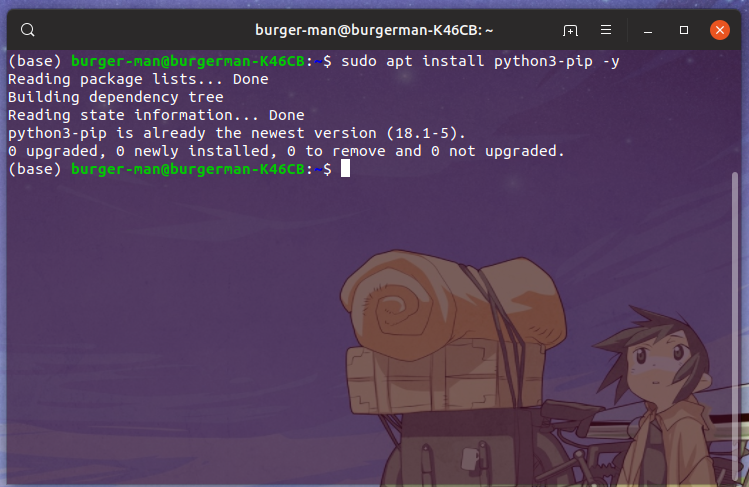
\includegraphics[width=1\textwidth]{figures/installpip.png}
\caption{Gambar instal pip}
\label{installpip}
\end{figure}

\end{enumerate}

\section{Setting Environment}
\subsection{Windows (Windows 10)}
\begin{enumerate}
\item Buka file explorer
\item Klik kanan pada This pc, lalu pilih properties
\begin{figure}[H]
    \centering
    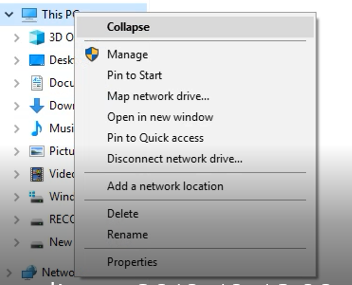
\includegraphics[scale=0.7]{figures/properties}
    \caption{\textit{Properties}}
    \label{Environment1}
\end{figure}
\item Pilih menu Advanced system settings
\begin{figure}[H]
    \centering
    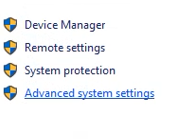
\includegraphics[scale=0.7]{figures/advanced}
    \caption{\textit{Advanced system settings}}
    \label{Environment2}
\end{figure}
\item Pilih Environment Variables
\begin{figure}[H]
    \centering
    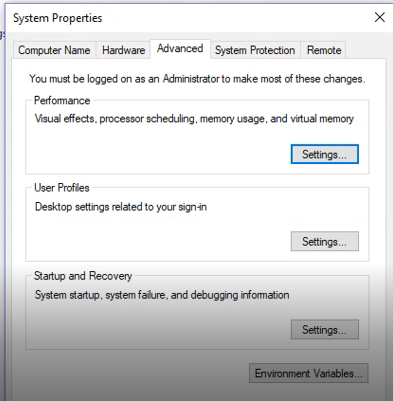
\includegraphics[scale=0.7]{figures/environment}
    \caption{\textit{Environment Variables}}
    \label{Environment3}
\end{figure}
\item Pilih Path
\begin{figure}[H]
    \centering
    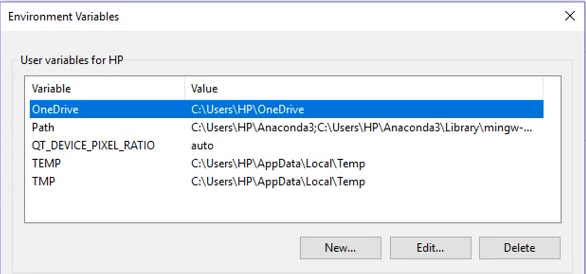
\includegraphics[scale=0.7]{figures/path}
    \caption{\textit{Path}}
    \label{Environment4}
\end{figure}
\item lalu pilih environment variable yang ingin ditambahkan, klik OK
\begin{figure}[H]
    \centering
    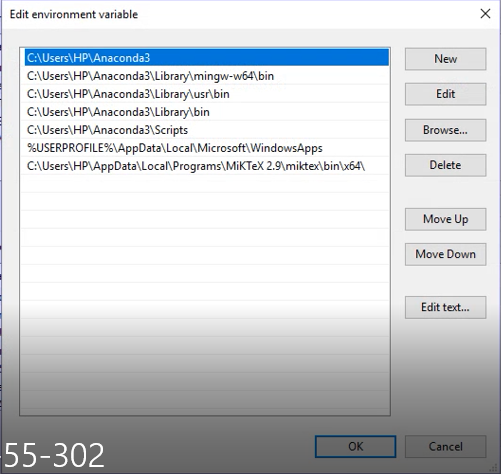
\includegraphics[scale=0.7]{figures/ok}
    \caption{\textit{Edit Environment Variable}}
    \label{Environment5}
\end{figure}
\end{enumerate}

\subsection{Linux (Ubuntu 19.04)}
\begin{enumerate}

\item pertama kita buka terminal kita lalu ketikkan perintah export PYTHONPATH=\$PYTHONPATH:pathinstallasipythonkalian contoh seperti gambar \ref{setpath}, lalu enter
\begin{figure}[H]
\centering
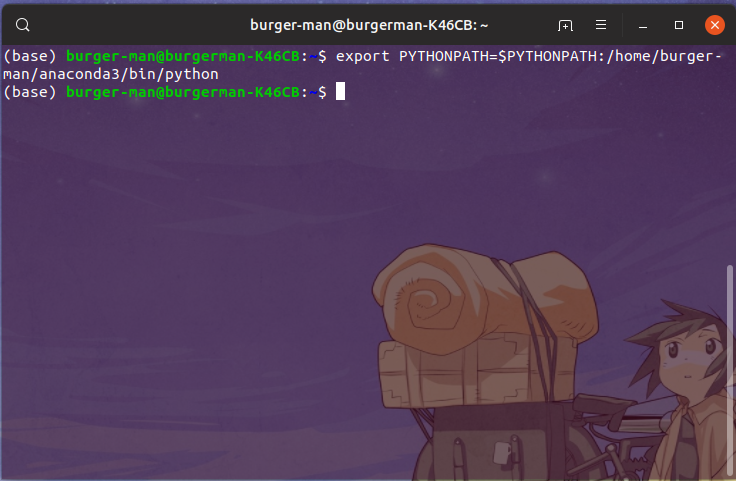
\includegraphics[width=1\textwidth]{figures/setpath.png}
\caption{Gambar setpath}
\label{setpath}
\end{figure}

\end{enumerate}

\section{Command Line Interface/Interpreter}
\subsection{Windows (Windows 10)}
\begin{enumerate}
\item Buka command prompt lalu ketikkan python
\item Buatlah perintah print, input, perkalian, dan pembagian
\item Bisa juga menjalankan file .py yang telah dibuat di IDE dengan cara python namafile.py, lalu klik enter
\begin{figure}[H]
    \centering
    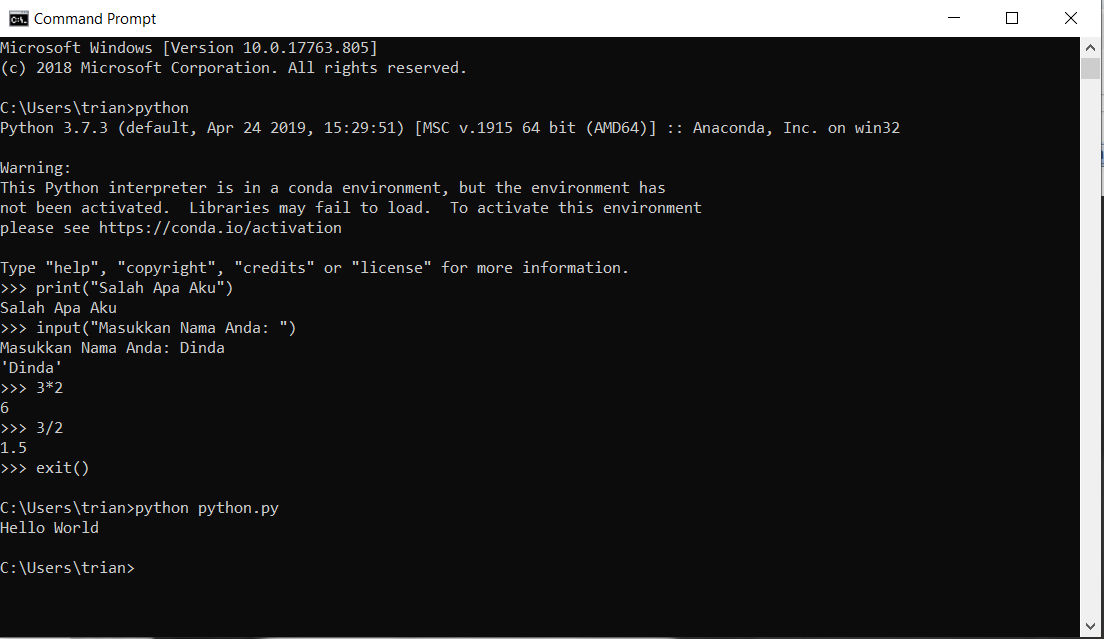
\includegraphics[scale=0.5]{figures/cli (2)}
    \caption{\textit{CLI in Command Prompt}}
    \label{CLI}
\end{figure}
\end{enumerate}

\subsection{Linux (Ubuntu 19.04)}
Untuk menjalankan perintah CLI cukup mudah yaitu sebagai berikut

\begin{enumerate}

\item Buka terminal lalu ketikkan \textbf{python \textit{namafile}.py} seperti gambar ~\ref{cli}, lalu enter
\begin{figure}[H]
\centering
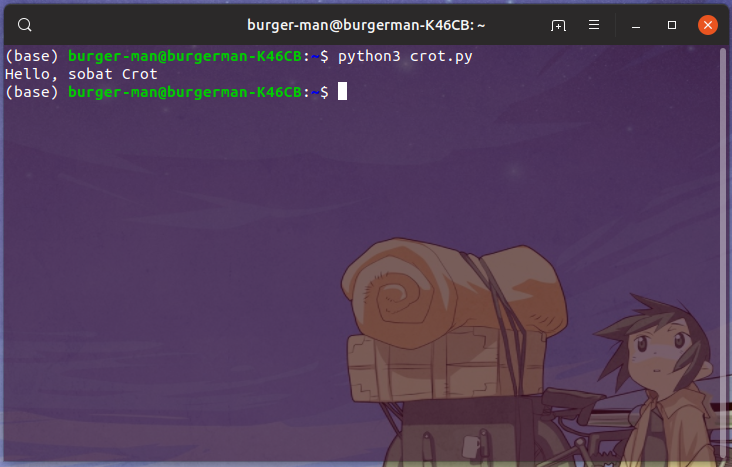
\includegraphics[width=1\textwidth]{figures/cli.png}
\caption{Gambar running script dengan CLI}
\label{cli}
\end{figure}

\end{enumerate}

\chapter{Judul Bagian Kedua}
\section{Variabel}
Variabel adalah sebuah tempat untuk menampung value dimemori, dapat dimisalkan seperti sebuah ruangan atau wadah, variabel dibagi dua berdasarkan ruang lingkup yaitu variable lokal dan global, untuk menentukan variabel global atau lokal itu tergantung dari tempat dideklarasikannya variabel pada program yang sedang dibuat. Variabel global yaitu variabel yang dapat diakses di semua lingkup dalam program yang sedang dibuat, dalam kata lain variabel global ini dapat dikenali oleh semua fungsi dan prosedur, sementara variabel lokal yaitu variabel yang dapat diakses hanya di lingkup khusus, dalam kata lain variabel lokal ini hanya bisa diakses pada fungsi/prosedur dimana variabel itu dideklarasikan.
\par
Berikut merupakan standar-standar dalam penulisan variabel:
\begin{enumerate}
\item Nama variabel diawali dengan huruf atau garis bawah, contoh: nama, \_nama, namaKu, nama\_variabel.
\item Karakter selanjutnya dapat berupa huruf, garis bawah atau angka, contoh: \_\_nama, nama1, p1.
\item  Nama variabel tidak boleh diawali dengan angka
\item Karakter bersifat case-sensitive (huruf besar dan huruf kecil dibedakan), contoh: Nama dan NAMA keduanya memiliki arti yang berbeda dan merupakan variabel yang berbeda.
\item Nama variabel tidak boleh menggunakan kata kunci yang ada pada bahasa pemrograman python, contoh: if, else, while
\end{enumerate}

\section{Input dan Output}
Input \& output bertujuan agar pengguna dan program dapat berinteraksi,Perintah input() berguna untuk meminta inputan dari user, sehingga memungkinkan user untuk menginputkan data.\\
Perintah print() berguna untuk menampilkan output dari data yang diinputkan oleh user, sehingga data yang diinputkan user dapat ditampilkan ke layar.
\par
Contoh dari penggunaan input dan output adalah sebagai berikut:
\begin{lstlisting}[language=Python]
#Input yang ditujukan untuk user
nama=”informatics research center” 

#output yang didapatkan user
print(“Halo”, nama, ”selamat datang ”)
\end{lstlisting}

\section{Operasi Aritmatika}
Python memiliki operasi aritmatika, antara lainnya seperti :
\begin{enumerate}
\item penjumlahan (+)
\item pengurangan (-)
\item perkalian (*)
\item pembagian (/)
\item sisa bagi/modulus (\%)
\item pemangkatan (**)
\end{enumerate}
Penggunaan dari simbol simbol ini sama hal nya dengan fungsi aritmatika pada umumnya.

\section{Perulangan}
Dalam membuat sebuah program, terkadang kita memerlukan satu baris atau satu blok kode yang sama secara berulang, disini fungsi perulangan dipakai sehingga kita tidak perlu menulis baris atau blok kode yang sama secara terus menerus, dalam python perulangan dibagi menjadi 2, yaitu for dan while.

\subsection{For}
For merupakan perulangan yang akan mengulang kondisi true sampai batas yang telah ditentukan,  biasanya digunakan untuk perulangan yang mana parameter pengulangannya menggunakan list atau range. Berikut ini merupakan contoh penggunakan sintaks perulangan for.
\begin{lstlisting}[language=Python]
for i in range (0 ,10): 
		print( i )
\end{lstlisting}

\subsection{While}
While merupakan perulangan yang akan terjadi apabila kondisinya True, perulangan akan terus berjalan hingga diperoleh kondisi False.erikut ini merupakan contoh penggunakan sintaks perulangan while.
\begin{lstlisting}[language=Python]
#perulangan while
hitung = 0 
while (hitung < 9): 
  	print (’hitungan ke :’, hitung) 
  	hitung = hitung + 1
 
print ("Good bye!")
\end{lstlisting}

\section{Kondisi}
Pengambilan keputusan kadang diperlukan dalam sebuah program untuk menentukan tindakan apa yang akan dilakukan sesuai dengan kondisi yang terjadi, contoh kasus misalkan ada seorang anak bernama idam, seorang manusia yang membutuhkan makan, jika idam lapar maka idam akan makan. Maka dapat dijabarkan seperti dibawah ini :\\
\\
Kondisi, jika : \\
Idam lapar \\
Maka : \\
Idam akan makan\\
Namun terkadang kondisi juga diberikan tambahan opsi sebuah kondisi tambahan, misalkan jika idam makan maka idam kenyang, namun jika tidak maka idam akan kelaparan. Penjabarannya dapat dilihat sebagai berikut :\\
\\
Kondisi, jika :\\
 Idam makan \\
 Maka : \\
 Idam akan kenyang \\
 Jika tidak : \\
 Idam akan kelaparan\\
Contoh diatas dapat ditulis dalam sintax python dengan menggunakan kondisi, pengkondisiian dalam python dibagi menjadi 4, yaitu : IF, IF ELSE, ELIF, nested IF. Berikut merupakan pembahasannya.

\subsubsection{IF}
 IF  adalah suatu struktur yang memiliki suatu perlakuan jika terjadi suatu kondisi. Akan tetapi, tidak terjadi sesuatu yang lain atau terjadi apa-apa ketika berada di dalam luar kondisi tersebut. IF hanya menjalankan satu kondisi dan menampilkan satu output. Contoh: kondisi dimana variabel a lebih besar dari variabel b, maka tampilkan hasil bahwa a lebih besar dari b.
\begin{lstlisting}[language=Python]
#if statement 
a = 330 
b = 200 
if a > a: 
	print("a lebih besar dari b")
\end{lstlisting}

\subsubsection{IF ELSE}
IF ELSE digunakan apabila kondisi yang terjadi bernilai salah, maka lakukan else. Contoh: kondisi dimana variabel a lebih besar dari variabel b, maka jika b lebih besar dari a, tampiilkan hasil b lebih besar dari a, jika salah maka tampilkan a lebih besar dari pada b
\begin{lstlisting}[language=Python]
 #else 
a = 200 
b = 33 
if b > a: 
	print("b is greater than a") 
else: 
	print("a is greater than b")
\end{lstlisting}

\subsubsection{ELIF}
Kondisi ELIF merupakan suatu strktur logika majemuk yang memiliki banyak pilihan aksi terhadap berbagai kemungkinan kejadian yang terjadi. ELIF digunakan apabila kondisi pertama tidak benar maka lakukan kondisi lain (alternatif). Contoh: kondisi dimana variabel a sama dengan variabel b, maka jika b lebih besar dari a, tampiilkan hasil b lebih besar dari a, namun jika a dan b bernilai sama, maka tampilkan a sama dengan b
\begin{lstlisting}[language=Python]
#elif 
a = 33 
b = 33 
if b > a: 
 	print("b lebih besar dari a") 
elif a == b: 
 	print("a sama dengan b")
\end{lstlisting}

\subsubsection{Nested IF}
Nested if merupakan if didalam if (if bersarang), terdapat dua if didalam satu kondisi. Contoh: variabel x sama dengan 41, kondisi pertama yaitu jika x besar dari 10 maka tampilkan lebih besar dari 10, kondisi kedua yaitu jika x besar dari 20, maka tampilkan lebih besar dari 20, jika salah maka tampilkan tidak melebihi 20.
\begin{lstlisting}[language=Python]
#nested if 
x = 41
 
if x > 10: 
 print("lebih besar dari 10,") 
 if x > 20: 
	 print("lebih besar dari 20!") 
 else: 
	 print("tidak melebihi 20.")
\end{lstlisting}

\section{Error}
\begin{enumerate}
\item NameError, terjadi apabila kode mengeksekusi nama yang tidak terdefenisikan. Contoh:
\begin{lstlisting}
nama = "Dinda Majesty"
print(Nama)
\end{lstlisting}

Maka akan menghasilkan output NameError: name ’Nama’ is not defined. error ini dapat diatasi dengan mengubah variabel yang di print sesuai dengan variabel yang didefenisikan, karena penulisan pada pyton bersifat case-sensitive

\item SyntaxError, terjadi apabila kode python mengalami kesalahan saat penulisan. Contoh: menuliskan variabel yang didahului angka (1nama = ”Dinda Majesty”) maka akan muncul eror SyntaxError: invalid syntax. error ini dapat diatasi dengan memperhatikan tata cara penulisan kode pada bahasa pemrograman python.

\item Logic error merupakan kesalahan yang terjadi karena kesalahan pembacaan data pada command perintah seperti data tidak terbaca atau tidak ada, dan tidak sesuai dengan aturannya. Contoh kesalahan tipe data yaitu 
\begin{lstlisting}
a=’4’ 
b=6 

print(a+b)
\end{lstlisting}


\item TypeError, terjadi apabila kode melakukan operasi atau fungsi terhadap tipe data yang tidak sesuai. Contoh: melakukan penjumlahan terhadap tipe data string dan integer. eror ini dapat diatasi dengan mengubah tipe data string menjadi integer.
\begin{lstlisting}
a = "10"
b = 5

print(a + b)
\end{lstlisting}
Maka akan menghasilkan output eror TypeError: can only concatenate str (not ”int”) to str

\item IdentationError, terjadi apabila kode perulangan atau pengkondisian tidak menjorok kedalam (tidak menggunakan identasi), error ini dapat diatasi dengan menambahkan tab atau spasi. Contoh
\begin{lstlisting}
a = 200 
b = 330 

if b > a: 
print("b lebih besar dari a")
\end{lstlisting}
Maka akan menghasilkan output eror IndentationError: expected an indented block
\end{enumerate}

\section{Try Except}
Try Except merupakan salah satu bentuk penangan error di dalam bahasa pemrograman python, perintah try except ini memiliki fungsi untuk menangkap sebuah error dan tetap menjalankan program kita, sehingga program yang sedang dijalankan akan mengeksekusi program hingga akhir. Contohnya terdapat pada listing berikut
\begin{lstlisting}[language=Python]
a="1"
b=2

try:
	a+b
except:
	print("Error, kedua tipe data berbeda")
\end{lstlisting}

\chapter{Fungsi dan Kelas}
\section{Teori}
\subsection{Fungsi}
Fungsi adalah sebuah blok kode yang memiliki nama fungsi dan kode program didalamnya jika dijalankan maka fungsi itu akan mengembalikan nilai. Fungsi dapat dipanggil berkali-kali sesuai dengan nama fungsi yang telah didefenisikan. Fungsi memiliki nilai kembalian (return). Contoh fungsi
\begin{lstlisting}[language=Python]
def nambahinAngka(angka1, angka2): 
	hasil = angka1 + angka2 
	return hasil
\end{lstlisting}

Apabila kita dapat memberikan nilai ke angka1 dan angka2, dan apa bila sudah diberi nilai dan program sudah dijalankan, maka program pun akan mengembalikan nilai berupa hasil dari penjumlahan angka 1 dan angka 2.

\section{Package}
Package merupakan sekumpulan modul yang dikemas oleh programmer dengan tujuan agar mempermudah dalam pembuatan kode program. Kita dapat membuat sebuah kode program atau fungsi didalamnya dan dapat secara mudah menggunakan kode program itu dengan cara memanggilnya pada kode program lainnya atau import package. Contoh nya adalah sebagai berikut
\begin{lstlisting}[language=Python]
def my_biodata(nama, umur): 
	bio = "nama saya " + nama + " umur saya " + umur 
	return bio 

def my_study(kampus, prodi): 
	study = "saya berkuliah di " + kampus + " program studi " + prodi
	return study
\end{lstlisting}
Kode diatas merupakan isi dari file fungsi.py, sedangkan saya ingin menjalankan program fungsi.py pada main.py sehingga kode program pada file main.py akan dituliskan seperti berikut:
\begin{lstlisting}[language=Python]
import fungsi
nama = "Dinda Majesty" 
umur = "19 Tahun" 
biodata = my_biodata(nama, umur) 
print(biodata)

kampus = "Politeknik Pos Indonesia" 
prodi = "D4-Teknik Informatika" 
kuliah = my_study(kampus, prodi) 
print(kuliah)
\end{lstlisting}
Kode program pada file main.py akan mengimport kode program yang ada pada file fungsi.py, sehingga dengan adanya fungsi dan package kita dapat dengan mudah melakukan pemanggilan fungsi yang telah kita deskripsikan sebelumnya, walaupun berada pada file python yang berbeda.

\section{Class, Object, Atribute, and Method}
Class atau Kelas merupakan sebuah blueprint/kerangka dari objek yang berisi fungsi dan dibuat untuk mendefenisikan objek dengan atribut yang sesuai dengan kelas yang telah dibuat yang nantinya akan diinisiasikan. Objek adalah sebuah wujud yang dapat kita lakukan perintah sesuai dengan methodnya,Sebuah kelas harus memiliki objek yang nantinya akan di kodekan sesuai dengan fungsi yang telah dibuat pada kelas, tanpa adanya objek sebuah kelas tidak akan bisa menjalankan fungsi-fungsi didalamnya. Atribut berisi variabel yang memiliki tipe data dan dapat kita berikan pada objek, atribut ada 2 yaitu kelas atribut dan instansi atribut, perbedaannya hanya di letak, kalau kelas atribut ada di bawah kelas, dan instansi atribut ada didalam fungsi, atribut itu sebuah variabel yang dimiliki oleh parentnya seperti fungsi atau class. .Method merupakan kode program yang berisi tindakan atau perintah untuk menjalankan objek.
\begin{lstlisting}[language=Python]
class Fungsi(object): 

def Nama(self, namakamu):
self.kamu = namakamu
\end{lstlisting}

\section{Pemanggilan Class}
Pemanggilan library kelas dapat dilakukan dengan cara import dan membuat objek dari kelas tersebut. Contohnya, kita memiliki file python yang diberi nama ngitung dan didalamnya terdapat class Ngitung yang memiliki banyak fungsi didalamnya. Untuk melakukan pemanggilan class maka kita bisa mengetikkan kode seperti berikut.
\begin{lstlisting}[language=Python]
import Fungsi
\end{lstlisting}

\section{Pemakaian Package Fungsi Apabila File Didalam Folder}
Pemakaian Package fungsi apabila file terdapat didalam sebuah folder maka kita bisa menggunakan from folder import file dan from file import fungsi. Contohnya, kita memiliki folder src yang didalamnya terdapat file fungsi.py dan didalam fungsi.py terdapat fungsi Berhitung, untuk mengimportkan fungsi maka kita dapat mengetikkan kode seperti berikut.
\begin{lstlisting}[language=Python]
from src import fungsi 
from fungsi import Berhitung
\end{lstlisting}

\section{Pemakaian Package Kelas Apabila File didalam Folder}
Pemakaian package kelas apabila file terdapat didalam sebuah folder maka kita bisa menggunakan from folder import file dan from file import kelas. Contohnya, kita memiliki folder src yang didalamnya terdapat file fungsi.py dan didalam fungsi.py terdapat kelas Ngitung, maka untuk melakukan import kelas kita dapat mengetikkan kode sebagai berikut.
\begin{lstlisting}[language=Python]
from src import fungsi 
Kelas = fungsi.Nama(namakamu)
\end{lstlisting}



\bibliographystyle{IEEEtran} 
%\def\bibfont{\normalsize}
\bibliography{references}


%%%%%%%%%%%%%%%
%%  The default LaTeX Index
%%  Don't need to add any commands before \begin{document}
\printindex

%%%% Making an index
%% 
%% 1. Make index entries, don't leave any spaces so that they
%% will be sorted correctly.
%% 
%% \index{term}
%% \index{term!subterm}
%% \index{term!subterm!subsubterm}
%% 
%% 2. Run LaTeX several times to produce <filename>.idx
%% 
%% 3. On command line, type  makeindx <filename> which
%% will produce <filename>.ind 
%% 
%% 4. Type \printindex to make the index appear in your book.
%% 
%% 5. If you would like to edit <filename>.ind 
%% you may do so. See docs.pdf for more information.
%% 
%%%%%%%%%%%%%%%%%%%%%%%%%%%%%%

%%%%%%%%%%%%%% Making Multiple Indices %%%%%%%%%%%%%%%%
%% 1. 
%% \usepackage{multind}
%% \makeindex{book}
%% \makeindex{authors}
%% \begin{document}
%% 
%% 2.
%% % add index terms to your book, ie,
%% \index{book}{A term to go to the topic index}
%% \index{authors}{Put this author in the author index}
%% 
%% \index{book}{Cows}
%% \index{book}{Cows!Jersey}
%% \index{book}{Cows!Jersey!Brown}
%% 
%% \index{author}{Douglas Adams}
%% \index{author}{Boethius}
%% \index{author}{Mark Twain}
%% 
%% 3. On command line type 
%% makeindex topic 
%% makeindex authors
%% 
%% 4.
%% this is a Wiley command to make the indices print:
%% \multiprintindex{book}{Topic index}
%% \multiprintindex{authors}{Author index}

\end{document}


